%\documentclass[tikz, border=5pt]{standalone}
\begin{document}
	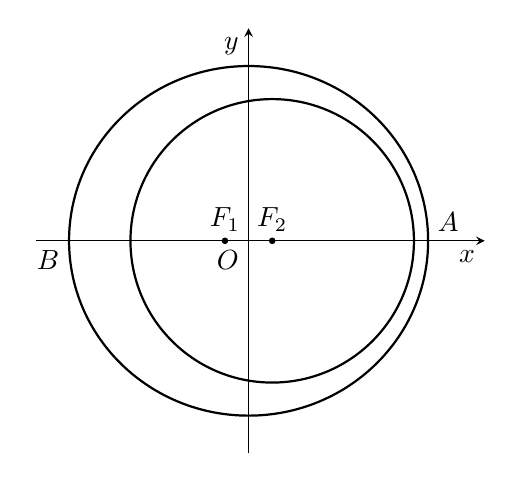
\begin{tikzpicture}[>=stealth, scale=0.6]
		% 3. 绘制椭圆
		\draw[thick] (0.5,0) circle(3);
		\draw[thick] (0,0) ellipse ({3.8} and {3.7});
		
		% 4. 绘制坐标轴
		\draw[->] (-4.5,0) -- (5,0) node[below left] {$x$};
		\draw[->] (0,-4.5) -- (0,4.5) node[below left] {$y$};
		\node at (0,0) [below left] {$O$}; % 原点
		
		% 5. 标记顶点与焦点
		\node at (-3.8,0) [below left] {$B$};   % 左顶点
		\node at (3.8,0)  [above right] {$A$};  % 右顶点
		\fill (-0.5,0) circle (2pt) node[above] {$F_1$}; % 左焦点
		\fill (0.5,0) circle (2pt) node[above] {$F_2$}; % 右焦点
		
	\end{tikzpicture}
\end{document}
